\documentclass[margin,line]{res}

\usepackage{CJKutf8}

\usepackage{graphicx}
\usepackage{float}
\usepackage{tabularx}
\usepackage{hyperref}
\hypersetup{
  colorlinks   = true, %Colours links instead of ugly boxes
  urlcolor     = blue, %Colour for external hyperlinks
  linkcolor    = blue, %Colour of internal links
  citecolor   = red %Colour of citations
}

\oddsidemargin -.5in
\evensidemargin -.5in
\textwidth=6.0in
\itemsep=0in
\parsep=0in
% if using pdflatex:
\setlength{\pdfpagewidth}{\paperwidth}
\setlength{\pdfpageheight}{\paperheight} 

\newenvironment{list1}{
  \begin{list}{\ding{113}}{%
      \setlength{\itemsep}{0in}
      \setlength{\parsep}{0in} \setlength{\parskip}{0in}
      \setlength{\topsep}{0in} \setlength{\partopsep}{0in} 
      \setlength{\leftmargin}{0.17in}}}{\end{list}}
\newenvironment{list2}{
  \begin{list}{$\bullet$}{%
      \setlength{\itemsep}{0in}
      \setlength{\parsep}{0in} \setlength{\parskip}{0in}
      \setlength{\topsep}{0in} \setlength{\partopsep}{0in} 
      \setlength{\leftmargin}{0.2in}}}{\end{list}}


\begin{document}
\begin{CJK*}{UTF8}{gbsn}

\name{苏道毕力格 \vspace*{.1in}}

\begin{resume}



%%%%%%%%%%%%%
%\section{\sc 个人信息}
%\vspace{.05in}
%\begin{tabularx}{\textwidth}{X r}
%博士后研究员 & 1987-09-10日生，蒙古族\\
%\href{http://www.acfr.usyd.edu.au/}{澳大利亚室外机器人中心(ACFR)}, \href{https://sydney.edu.au/}{{悉尼大学}}     &  +61(0)-410-891-777 \\            
%J04 - Rose Street BD, The University of Sydney & daobilige.su@sydney.edu.au \\         
%NSW 2006, Australia   & \\%{\it E-mail:} 
%%博士研究生 & 1987-09-10日生，蒙古族\\
%%自主系统研究中心（CAS）, 悉尼科技大学（UTS）      &  +61(0)-410-891-777 \\            
%%Building 11, Level 9, Room 300         & daobilige.su@gmail.com \\         
%%81 Broadway, Ultimo, NSW 2007, Australia  & \\%{\it E-mail:}  paciorek@stat.cmu.edu\\       
%%  & \\%{\it WWW:} www.stat.cmu.edu/\verb+~+paciorek \\     
%\end{tabularx}

%%%%%%%%%%%%
\section{\sc 个人信息}
\vspace{.05in}
\begin{tabularx}{\textwidth}{X r}
副教授 & 1987-09-10日生，蒙古族\\
\href{http://en.cau.edu.cn/}{中国农业大学 (CAU)}, \href{http://coe.cau.edu.cn/}{工学院}, 机电工程系     &  sudao@cau.edu.cn \\            
北京市海淀区清华东路17号中国农业大学东校区工学院447 & \\         
%NSW 2006, Australia   & \\%{\it E-mail:} 
%博士研究生 & 1987-09-10日生，蒙古族\\
%自主系统研究中心（CAS）, 悉尼科技大学（UTS）      &  +61(0)-410-891-777 \\            
%Building 11, Level 9, Room 300         & daobilige.su@gmail.com \\         
%81 Broadway, Ultimo, NSW 2007, Australia  & \\%{\it E-mail:}  paciorek@stat.cmu.edu\\       
%  & \\%{\it WWW:} www.stat.cmu.edu/\verb+~+paciorek \\     
\end{tabularx}



%%%%%%%%%%%%
\section{\sc 研究方向}
农业机器人, 人工智能, 深度学习, SLAM(同时定位与制图), 机器人导航, 机器人视觉/听觉


%%%%%%%%%%%%
\section{\sc 当前工作}
\begin{tabularx}{\textwidth}{X r}
%\href{http://www.uts.edu.au}{{\bf University of Sydney}}, Sydney, Australia  
{\bf 副教授}, &2020-09 - 至今\\
\end{tabularx}
%{\em Department of Statistics} 
\vspace*{-.1in}
\begin{list1}
\item[] \href{http://en.cau.edu.cn/}{中国农业大学 (CAU)}, \href{http://coe.cau.edu.cn/}{工学院}, 机电工程系, 北京, 中国
\end{list1}
\begin{figure}[H]
  \centering
  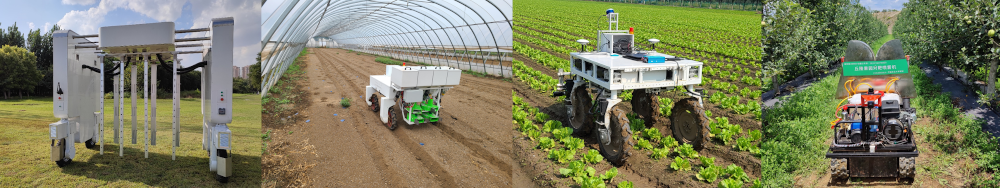
\includegraphics[width=0.99\columnwidth]{./figs/cau_robots_smallsize.png}
  %\caption{The architecture of non-bottleneck-1D block.}
  \label{fig:cau_robots}
\end{figure}

%%%%%%%%%%%%


%%%%%%%%%%%%
\section{\sc 教育背景}
\begin{tabularx}{\textwidth}{X r}
%\href{http://www.uts.edu.au}{{\bf University of Sydney}}, Sydney, Australia  
博士后研究员, &2017-03 - 2020-04\\
\end{tabularx}
%{\em Department of Statistics} 
\vspace*{-.1in}
\begin{list1}
\item[] \href{http://www.acfr.usyd.edu.au/}{澳大利亚室外机器人中心 (ACFR)}, %\\ {\it Expected:} Jan. 2017
\href{https://sydney.edu.au/}{{悉尼大学}}, 悉尼, 澳大利亚
\begin{list2}
\vspace*{.05in}
\item 研究课题:  ``Intelligent Perception Systems for Agriculture and the Environment'' (农业环境的智能感知系统开发)
%\item Dissertation Topic:  ``Hierarchical Models for Multiple Ratings
%  in Performance-Based\\ \hspace*{1.23in} Student Assessments.'' 
\item 导师: \href{http://sydney.edu.au/engineering/people/salah.sukkarieh.php}{Prof. Salah Sukkarieh} (澳大利亚科学院(\href{https://www.atse.org.au/}{ATSE})院士), %\href{http://sydney.edu.au/engineering/people/james.underwood.php}{Dr. James Underwood}
\item \textbf{参与研发的机器人}: \href{https://confluence.acfr.usyd.edu.au/display/AGPub/Our+Robots}{Ladybird, RIPPA, Digital Farmhand, Shrimp} (\href{https://sydney.edu.au/engineering/our-research/robotics-and-intelligent-systems/australian-centre-for-field-robotics/agriculture-and-the-environment.html}{其他链接})
\end{list2}
\end{list1}

\begin{figure}[H]
  \centering
  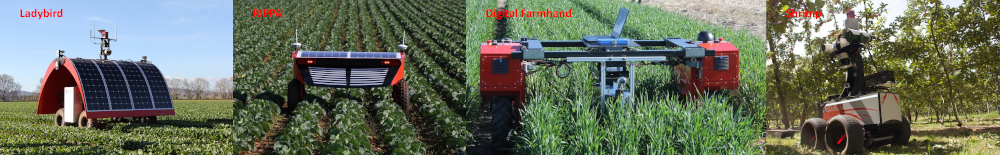
\includegraphics[width=0.99\columnwidth]{./figs/ladybird_rippa_digitalfarmhand_shrimp_smallsize.png}
  %\caption{The architecture of non-bottleneck-1D block.}
  \label{fig:ladybird_rippa_digitalfarmhand_shrimp}
\end{figure}

\begin{tabularx}{\textwidth}{X r}
\href{http://www.uts.edu.au}{{\bf 悉尼科技大学(UTS)}}, 悉尼, 澳大利亚  &2013-03 - 2017-03\\
\end{tabularx}
%{\em Department of Statistics} 
\vspace*{-.1in}
\begin{list1}
\item[] 博士研究生， 机器人领域， \href{http://www.cas.uts.edu.au}{自主系统研究中心（CAS）}%\\ %{\it 预期毕业时间:} 01/2017
\begin{list2}
\vspace*{.05in}
\item 博士课题:  ``Robotic Sound Source Mapping using Microphone Arrays'' 
%\item Dissertation Topic:  ``Hierarchical Models for Multiple Ratings
%  in Performance-Based\\ \hspace*{1.23in} Student Assessments.'' 
\item 导师: \href{http://www.uts.edu.au/staff/jaime.vallsmiro}{A/Prof. Jaime Valls Miro}
\item 副导师:  \href{http://www.uts.edu.au/staff/teresa.vidalcalleja}{Dr. Teresa Vidal Calleja}
\end{list2}
\end{list1}

\begin{tabularx}{\textwidth}{X r}
\href{http://emaro.irccyn.ec-nantes.fr/}{{\bf EMARO} (欧洲先进机器人硕士(EM双学位联合培养项目))} &2010-10 - 2012-10\\
\end{tabularx}
%{\em Department of Mathematics and Statistics} 
\vspace*{-.1in}
\begin{list1}
\item[] 热那亚大学, 意大利 (2011-10 - 2012-10)
\begin{list2}
\vspace*{.05in}
\item 自动化硕士学位, GPA: 92/100
\end{list2}
\begin{list2}
\vspace*{.05in}
\item 硕士课题 完成与 日本庆应大学 (Apr, 2012 - Sep, 2012)\\
硕士课题: Designing Real-Time Robot Audition System (实时机器人听觉系统的设计)\\
导师: Prof. Nozumo Hamada
\end{list2}
\end{list1}
\begin{list1}
\item[] 华沙理工大学, 波兰 (2010-10 - 2011-07)
\begin{list2}
\vspace*{.05in}
\item 自动化与机器人硕士学位, GPA: 81.5/100
\end{list2}
\end{list1}

\begin{tabularx}{\textwidth}{X r}
\href{http://www.zju.edu.cn/english/}{{\bf 浙江大学}}, 中国   &2006-09 - 2010-07\\
\end{tabularx}
%{\em Department of Mathematics and Statistics} 
\vspace*{-.1in}
\begin{list1}
\item[] 机械电子工程学士学位, GPA: 3.63/4.0 (专业课GPA: 3.76/4.0)
\end{list1}



%%%%%%%%%%%%
\section{\sc 项目经历} 

\begin{itemize}

\item {\bf 无农药除草机器人的智能感知系统开发}\\
2018-09 - 至今, ACFR, 悉尼大学.\\
%Development of a deep learning based method for semantic segmentation of weed against crop using TensorFlow, C++ and ROS. \\
基于深度学习的农作物与杂草的实时语义分割，TensorFlow, C++ and ROS. \\
(企业保密协议项目)\\
\begin{figure}[H]
  \centering
  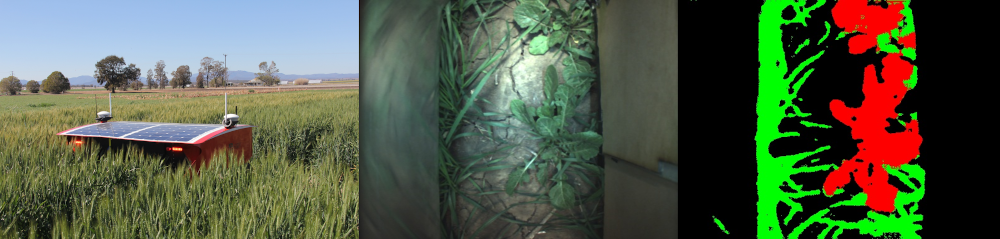
\includegraphics[width=0.9\columnwidth]{./figs/clyde_seg_smallsize.png}
\end{figure}

\item {\bf %Intelligent Perception for Robotic Precision Spray of Vegetable Crops 
蔬菜精确喷洒农药机器人的智能感知系统开发}\\
2017-09 - 2018-09, ACFR, 悉尼大学.\\
%Development of a deep learning based method to detect and track vegetable crops and leaf segmentation and localization for precision spray using TensorFlow.
基于深度学习的蔬菜识别,跟踪, 菜叶分割和定位.用于农业机器人对蔬菜精确喷洒农药.\\
%The method allow an agricultural robot to accurately spray individual leaves of crops. \\
(企业保密协议项目)\\
\begin{figure}[H]
  \centering
  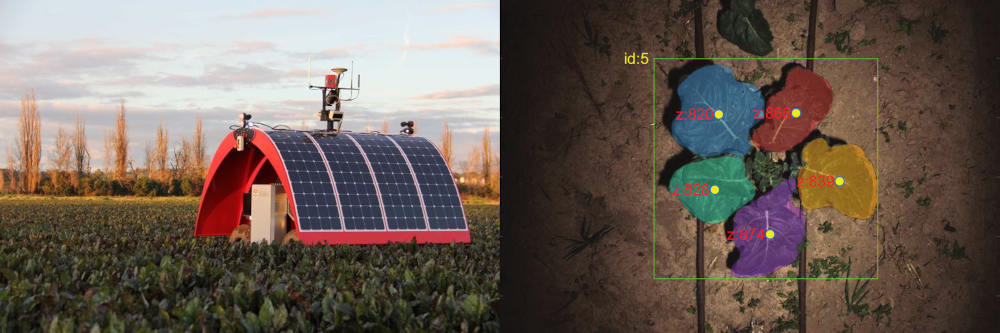
\includegraphics[width=0.62\columnwidth]{./figs/ladybird_leaf_seg_smallsize.png}
\end{figure}

\item {\bf 基于3D激光雷达的农业机器人在果树林中的同时定位与制图(SLAM)}\\
2017-03 - 2017-09, ACFR, 悉尼大学.\\
基于Velodyne3D激光雷达点云的同时定位与制图(SLAM)算法的开发.用于农业机器人在果树林中的定位与制图.\\
(企业保密协议项目)\\
\begin{figure}[H]
  \centering
  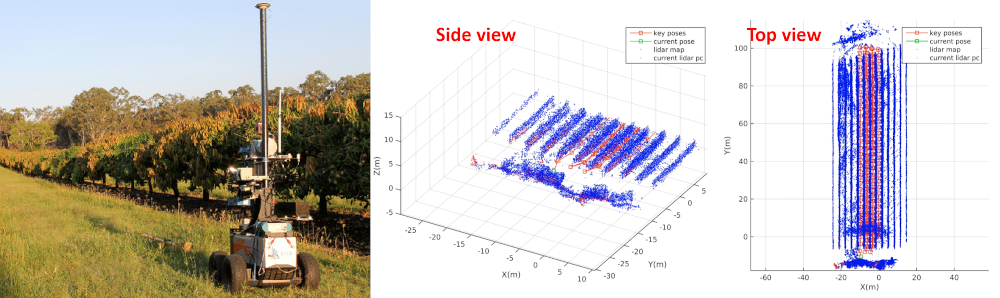
\includegraphics[width=0.9\columnwidth]{./figs/shrimp_lidar_loc_smallsize.png}
\end{figure}

\item {\bf 基于Invariant卡尔曼滤波的视觉惯性制导系统(VINS) 算法的开发}\\
2016-09 - 2017-03, CAS, UTS.\\
基于在流形上面优化的视觉惯性制导系统(VINS)SLAM后段的开发, Matlab.\\
基于MSCKF卡尔曼滤波的视觉惯性制导系统后段的开发, Matlab.\\
图片特征提取,匹配和视觉场地识别, OpenCV and ORBSLAM前端.\\
\begin{figure}[H]
  \centering
  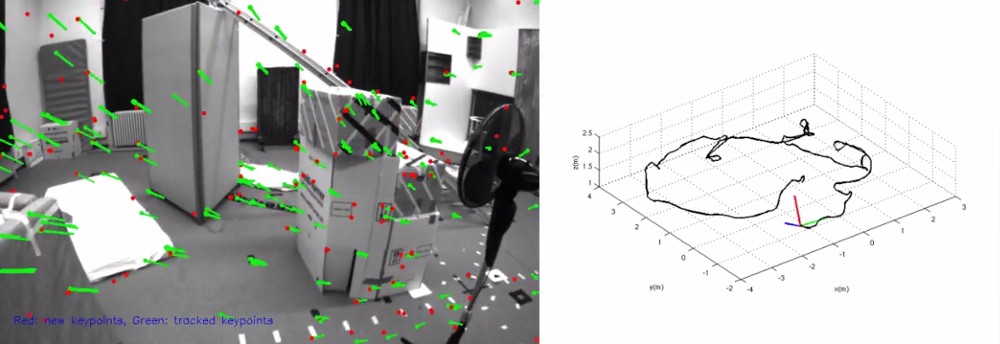
\includegraphics[width=0.7\columnwidth]{./figs/vins_paper_img_smallsize.png}
\end{figure}

\item {\bf 基于手持Kinect/PS3-Eye传感器的，融合3D视觉，声源的SLAM系统}\\
2015-09 - 至今, CAS, UTS.\\
基于视觉与声学信息融合的SLAM制图系统的开发，C++和Matlab(仿真).\\
基于OpenCV和ORBSLAM前端的，视觉特征点提取和匹配，图像识别.\\
基于逆深度，EKF滤波的声源位置的估计，基于g2o的声源位置的优化.\\
基于PCL和Octo Mapping的点云信息的处理.\\
相关视频: \href{https://youtu.be/QyqY2eIX1wk}{https://youtu.be/QyqY2eIX1wk}.\\
\begin{figure}[H]
  \centering
  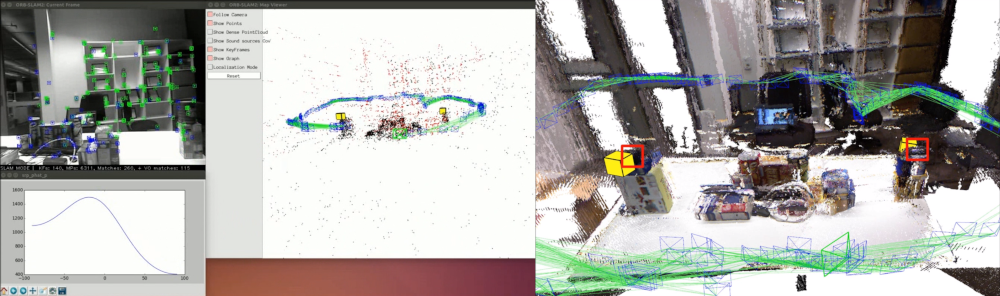
\includegraphics[width=0.7\columnwidth]{./figs/ssm_linear_smallsize.png}
\end{figure}

\item {\bf 基于Velodyne 3D激光扫描和Kinect RGBD相机的Husky机器人的SLAM系统}\\
2015-05 - 2015-09, HRI-JP.\\
Velodyne 3D激光扫描器与Microsoft Kinect与PC机之间接口的实现.\\
3D激光SLAM制图ROS包LOAM，与RGBD-SLAM ROS包的精细调参(运用C++和ROS).\\
(企业保密协议项目)\\

\item {\bf 基于安装有２D激光和麦克风矩阵的Turtlebot的室内声源定位}\\
2015-05 - 2015-09, HRI-JP.\\
外部传感器的安装与PC接口调试.\\
安装，调试和调节基于Hokoyu激光的2D SLAM ROS包（运用Hector SLAM, C++）.\\
基于麦克风矩阵的声源定位，光线追踪，声源聚类等（运用ROS, C++和Matlab）.\\
移动机器人轨迹优化，探索和优化观测值的移动（运用ROS, Python和Matlab）.\\
移动机器人的Gazebo仿真和RViz可视化.\\
\begin{figure}[H]
  \centering
  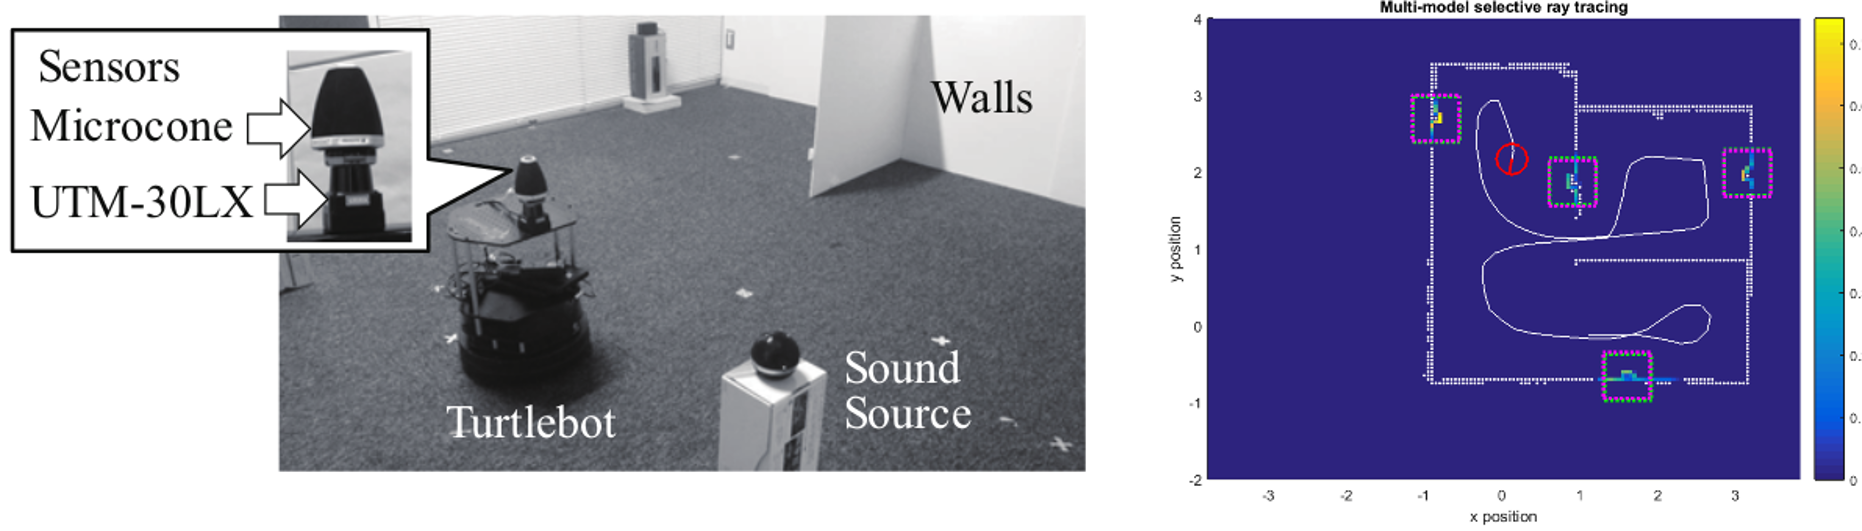
\includegraphics[width=0.8\columnwidth]{./figs/ssm_multi_model.png}
\end{figure}


\item {\bf GUTS智能跟踪移动机器人的硬件软件的设计}\\
2013-10 - 至今, CAS, UTS.\\
所有传感器相关硬件的设计，安装和调试（超声和红外传感器矩阵，无线RF传输器，车轮编码器和摄像头）和马达控制器的设计，安装和调试.\\
部分机械结构的设计（运用Solidworks）.\\
嵌入式微机的编程，PC接口设计，马达速度的PID控制（运用C/C++）.\\
高层软件的编程：传感器信号处理，基于机器学习的传感器概率模型的建立，机器人状态估计，机器人移动规划和可视化（运用ROS, C/C++, Python, GPy(Gaussian Process Python库), Matlab Robotics Toolbox, Rviz, V-Rep(仿真)）.\\
相关视频: \href{https://youtu.be/hjLQfrdelcs}{https://youtu.be/hjLQfrdelcs}.\\
\begin{figure}[H]
  \centering
  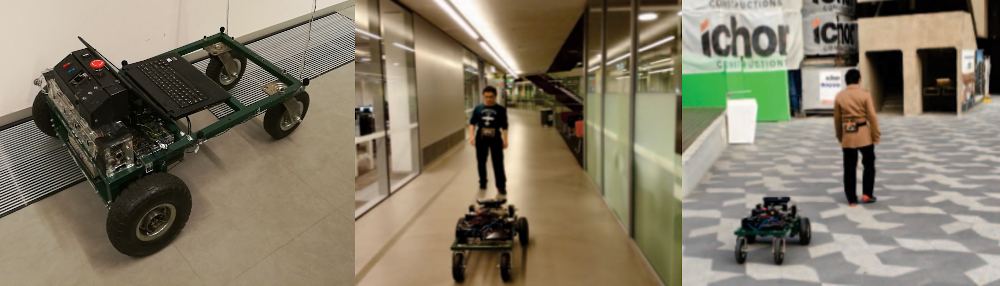
\includegraphics[width=0.9\columnwidth]{./figs/guts_tracking_smallsize.png}
\end{figure}

%\item {\bf 实时机器人听觉系统（语音识别和声源跟踪）的设计}\\
%2012-04 - 2012-08, 庆应大学.\\
%特征向量提取和基于机器学习的特征向量的建模（FMCC特征和Gaussian Mixture Model建模）.\\
%集成，调试和调节多通道麦克风矩阵驱动程序和其他接口实现（如蓝牙接口等）（运用C/C++）.\\ 
%麦克风矩阵的实时信号处理和声源DOA估计，实时鲁棒声源跟踪（运用ROS, C/C++）.\\
%相关视频: \href{http://youtu.be/xMn4iih-akE}{http://youtu.be/xMn4iih-akE}.\\

%\item {\bf Erasmus Mundus Scholarship} for Master study as EMARO, funded by European Union, Approx. 10 scholarships available for applications from all over the world (outside Europe), 2010-2012.
%
%\item {\bf Academic Excellent Scholarship} by Zhejiang University, China.
%\item {\bf 基于图像的自动拉丁字母的识别}\\
%2010-10 - 2011-01, 华沙理工大学.\\
%图像特征提取，贝叶斯监督性学习（运用openCV, ROS和C++）.\\

\end{itemize}






%%%%%%%%%%%%
\section{\sc 发表论文}
%Paciorek, C.J., J.S. Risbey, V. Ventura, and R.D.Rosen. 2002. Multiple indices of Northern Hemisphere Cyclone
%Activity, Winters 1949-1999. Journal of Climate 15:1573-1590.
%
%Paciorek, C.J., R. Condit, S.P. Hubbell, and R.B. Foster.  2000.
%The demographics of resprouting in tree and shrub species of a moist
%tropical forest.  Journal of Ecology 88:765-777.
%
%Paciorek, C.J., B.R. Moyer, R.A. Levin, and S.L. Halpern.  1995.
%Pollen consumption by hummingbird flower mite {\it Proctolaelaps
%  kirmsei} and possible fitness effects on {\it Hamelia patens}.
%Biotropica 27:258-262.  (author order determined by lot)  
\textbf{期刊论文}

\begin{enumerate}

\item \textbf{Daobilige Su}, He Kong, Salah Sukkarieh, and Shoudong Huagn, ``Necessary and Sufficient Conditions for Observability of SLAM-based Microphone Array Calibration and Sound Source Localization'', \textbf{under review} in \textit{IEEE Transactions on Robotics}, 2020. (2019 IF  \textbf{6.123})

\item \textbf{Daobilige Su}, Yongliang Qiao, He Kong, and Salah Sukkarieh, ``Real Time Detection of Inter-Row Ryegrass in Wheat Farm using Deep Learning'', \textbf{under review} in \textit{Biosystems Engineering}, 2019. (2019影响因子\textbf{2.983}, 中科院 2区, JCR 1区)

\item He Kong, Mao Shan, \textbf{Daobilige Su}, Yongliang Qiao, Abdullah Al-Azzawi, and Salah Sukkarieh, ``Filtering for Systems subject to Unknown Inputs without Apriori Initial Information'', \textbf{Online} in \textit{Automatica}, 2019. (2019影响因子\textbf{5.541}, 中科院 1区\textbf{Top期刊}, JCR 1区)

\item \textbf{Daobilige Su}, He Kong, and Salah Sukkarieh, ``Data Augmentation for Deep Learning based Semantic Segmentation and Crop-Weed Classification in Agricultural Robotics'', \textbf{under review} in \textit{Biosystems Engineering}, 2019. (2019影响因子\textbf{2.983}, 中科院 2区, JCR 1区)

\item Jasper Brown, \textbf{Daobilige Su}, He Kong, Salah Sukkarieh, and Eric Kerrigan. ``Improved Noise Covariance Estimation in Visual Servoing Using an Autocovariance Least-squares Approach'', \textbf{invited paper} to \textit{Mechatronics}, 2019. (2019影响因子\textbf{2.978}, 中科院 2区, JCR 1区)

\item {\bf Daobilige Su}, Teresa Vidal Calleja and Jaime Valls Miro, ``Simultaneous asynchronous microphone array calibration and sound source localisation'', {\it Autonomous Robots}, pp. 1-22, 2019. (2019影响因子\textbf{3.634}, 中科院 3区, JCR 1区)

% Yongliang Qiao, Salah Sukkarieh and Daobilige Su, Animal Sound Detection and Clustering using Manifold Regularized Deep Learning
%\item Yongliang Qiao, Salah Sukkarieh, {\bf Daobilige Su}*, ``Animal Sound Detection and Clustering using Manifold Regularized Deep Learning'', \textbf{accepted} in {\it Sensors}, 2018. (*通讯作者, 2018影响因子 \textbf{2.475}, JCR 2区)

% Su, Daobilige, Asher Bender, and Salah Sukkarieh. "Improved Cross-Ratio Invariant-Based Intrinsic Calibration of A Hyperspectral Line-Scan Camera." Sensors 18, no. 6 (2018): 1885.
\item {\bf Daobilige Su}, Asher Bender and Salah Sukkarieh, ``Improved Cross-Ratio Invariant-Based Intrinsic Calibration of A Hyperspectral Line-Scan Camera'', in {\it Sensors}, vol. 18 no. 6, pp. 1885, 2018. (2019影响因子\textbf{3.031}, 中科院 2区, JCR 1区)

% Wang, Mengmeng, Yong Liu, Daobilige Su, Yufang Liao, Lei Shi, and Jinhong Xu. "Accurate and Real-time 3D Tracking for the Following Robots by Fusing Vision and Ultra-sonar Information." IEEE/ASME Transactions on Mechatronics (2018).
\item Mengmeng Wang, Yong Liu, {\bf Daobilige Su}, Yufang Liao, Lei Shi, Jinhong Xu and Jaime Valls Miro, ``Accurate and Real-time 3D Tracking for the Following Robots by Fusing Vision and Ultrasonar Information'', in {\it IEEE/ASME Transactions on Mechatronics}, vol. 23 no. 3, pp. 997-1006, 2018. (2018影响因子\textbf{3.936}, 中科院 1区{\bf Top期刊}, JCR 1区)
\end{enumerate}

\textbf{会议论文}
\begin{enumerate}

\item Yongliang Qiao, \textbf{Daobilige Su}, He Kong, Salah Sukkarieh, Sabrina Lomax, and Cameron Clark. ``Data Augmentation for Deep Learning based Cattle Segmentation in Precision Livestock Farming'', \textbf{accepted} in \textit{2020 IEEE International Conference on Automation Science and Engineering (CASE 2020)}, 2020.

\item Yongliang Qiao, \textbf{Daobilige Su}, He Kong, Salah Sukkarieh, Sabrina Lomax, and Cameron Clark. ``BiLSTM-based Individual Cattle Identification for Automated Precision Livestock Farming'', \textbf{accepted} in \textit{2020 IEEE International Conference on Automation Science and Engineering (CASE 2020)}, 2020.

\item Yongliang Qiao, \textbf{Daobilige Su}, He Kong, Salah Sukkarieh, Sabrina Lomax, and Cameron Clark. ``Individual Cattle Identification Using a Deep Learning Based Framework'', in {\it AgriControl 2019}, pp. 318-323, 2019.

% Brown, Jasper, Daobilige Su, He Kong, Salah Sukkarieh, and Eric Kerrigan. "Improved Noise Covariance Estimation in Visual Servoing Using an Autocovariance Least-squares Approach."
%The 12th IFAC Conference on Control Applications in Marine Systems, Robotics, and Vehicles (CAMS 2019) and the first workshop on Robot Control (WROCO 2019)
\item Jasper Brown, \textbf{Daobilige Su}, He Kong, Salah Sukkarieh, and Eric Kerrigan. ``Improved Noise Covariance Estimation in Visual Servoing Using an Autocovariance Least-squares Approach'', in \textit{Joint 12th IFAC Conference on Control Applications in Marine Systems, Robotics, and Vehicles (CAMS 2019) and the first workshop on Robot Control (WROCO 2019)}, 2019. ({\bf Best Paper Award Finalist}).

% Wang, Min, Holger Voos, and Daobilige Su. "Robust Online Obstacle Detection and Tracking for Collision-Free Navigation of Multirotor UAVs in Complex Environments." In 2018 15th International Conference on Control, Automation, Robotics and Vision (ICARCV), pp. 1228-1234. IEEE, 2018.
\item Min Wang, Holger Voos and {\bf Daobilige Su}, ``Robust Online Obstacle Detection and Tracking for Collision-free Navigation of Multirotor UAVs in Complex Environments'', in {\it 2018 15th International Conference on Control Automation Robotics \& Vision (ICARCV 2018)}, pp. 1228-1234, 2018.(IE)

\item Kanzhi Wu*, Teng Zhang*, {\bf Daobilige Su}, Shoudong Huang, Gamini Dissanayake, ``An Invariant-EKF VINS Algorithm for Improving Consistency'', in {\it 2017 IEEE/RSJ International Conference on Intelligent Robots and Systems (\textbf{IROS 2017})}, pp. 1578-1585, 2017.
(* indicates equal contribution)(IE，\textbf{机器人国际顶级会议})

\item {\bf Daobilige Su}, Teresa Vidal Calleja and Jaime Valls Miro, ``Towards Real-Time 3D Sound Sources Mapping with Linear Microphone Arrays'', in {\it 2017 IEEE International Conference on Robotics and Automation (\textbf{ICRA 2017})}, pp. 1662-1668, 2017.
%2017. 
(Affiliated Video: \\ \href{https://youtu.be/Ry_i3kmvlHM}{{https://youtu.be/Ry\_i3kmvlHM}}, Open source code: \\ \href{https://github.com/daobilige-su/SSM_LinearArray}{{https://github.com/daobilige-su/SSM\_LinearArray}}) (IE，\textbf{机器人国际顶级会议})

\item Mengmeng Wang, {\bf Daobilige Su}, Lei Shi, Yong Liu and Jaime Valls Miro, ``Real-time 3D Human Tracking for Mobile Robots with Multisensors'', in {\it 2017 IEEE International Conference on Robotics and Automation (\textbf{ICRA 2017})}, pp. 5081-5087, 2017. (IE，\textbf{机器人国际顶级会议})

\item {\bf Daobilige Su}, Teresa Vidal Calleja and Jaime Valls Miro, ``Split Conditional Independent Mapping for Sound Source Localisation with Inverse-Depth Parametrisation'', in {\it 2016 IEEE/RSJ International Conference on Intelligent Robots and Systems (\textbf{IROS 2016})}, pp. 2000-2006, 2016. (Affiliated Video: \href{https://youtu.be/QyqY2eIX1wk}{{https://youtu.be/QyqY2eIX1wk}}) (IE，\textbf{机器人国际顶级会议})

\item {\bf Daobilige Su}, Keisuke Nakamura, Kazuhiro Nakadai and Jaime Valls Miro, ``Robust Sound Source Mapping using Three-layered Selective Audio Rays for Mobile Robots'', in {\it 2016 IEEE/RSJ International Conference on Intelligent Robots and Systems (\textbf{IROS 2016})}, pp. 2771-2777, 2016. (IE，\textbf{机器人国际顶级会议})

\item {\bf Daobilige Su}, Teresa Vidal Calleja and Jaime Valls Miro, ``Simultaneous asynchronous microphone array calibration and sound source localisation'', in {\it 2015 IEEE/RSJ International Conference on Intelligent Robots and Systems (\textbf{IROS 2015})}, pp. 5561-5567, 2015. (IE，\textbf{机器人国际顶级会议})

\item {\bf Daobilige Su}, Jaime Valls Miro and Teresa Vidal Calleja, ``Graph-SLAM Based Calibration of an Embedded Asynchronous Microphone Array for Outdoor Robotic Target Tracking'', in {\it Assistive Robotics: Proceedings of the 18th International Conference on CLAWAR 2015}, pp. 641-648, 2015. ({\bf Best Paper Award Finalist}).

\item {\bf Daobilige Su}, Jaime Valls Miro and Teresa Vidal Calleja, ``Real-time sound source localisation for target tracking applications using an asynchronous microphone array'', in {\it 2015 IEEE 10th Conference on Industrial Electronics and Applications (ICIEA 2015)}, pp. 1261-1266, 2015.(IE)

\item {\bf Daobilige Su}, Jaime Valls Miro and Teresa Vidal Calleja, ``Modelling in-pipe acoustic signal propagation for condition assessment of multi-layer water pipelines'', in {\it 2015 IEEE 10th Conference on Industrial Electronics and Applications (ICIEA 2015)}, pp. 545-550, 2015. ({\bf Best Paper Award Finalist}).(IE)

\item {\bf Daobilige Su}, Nalika Ulapane and Buddhi Wijerathna, ``An acoustic sensor based novel method for 2D localization of a robot in a structured environment'', in {\it 2015 IEEE 10th Conference on Industrial Electronics and Applications (ICIEA 2015)}, pp. 2024-2029, 2015.(IE)

\item {\bf Daobilige Su} and Jaime Valls Miro. ``An ultrasonic/RF GP-based sensor model robotic solution for indoors/outdoors person tracking'', in {\it 2014 13th International Conference on Control Automation Robotics \& Vision (ICARCV 2014)}, pp. 1662-1667, 2014.(IE)

\item Teresa Vidal Calleja, {\bf Daobilige Su}, Freek De Bruijn and Jaime Valls Miro, ``Learning spatial correlations for Bayesian fusion in pipe thickness mapping'', in {\it 2014 IEEE International Conference on Robotics and Automation (\textbf{ICRA 2014})}, pp. 683-690, 2014. (IE，\textbf{机器人国际顶级会议})

\item Jaime Valls Miro, Jeya Rajalingam, Teresa Vidal Calleja, Freek de Bruijn, Roger Wood, Dammika Vitanage, Nalika Ulapane, Buddhi Wijerathna and {\bf Daobilige Su}, ``A live test-bed for the advancement of condition assessment and failure prediction research on critical pipes'', in {\it Proceedings of the Leading-Edge Strategic Asset Management Conference (LESAM13)}. 2013.

\item {\bf Daobilige Su}, Masashi Sekikawa, Kazuo Nakazawa and Nozomu Hamada, ``Novel scheme of real-time direction finding and tracking of multiple speakers by robot-embedded microphone array'', in {\it the 1st International Conference on Robot Intelligence Technology and Applications (RITA 2012)}, 2012.

\end{enumerate}

%%%%%%%%%%%%
\section{\sc 其他学术经历}

\begin{tabularx}{\textwidth}{X r}
{\bf 暑期学校} & 2015-02\\
\end{tabularx}
\begin{itemize}
\item[] \href{http://rp-www.cs.usyd.edu.au/~mlss/}{2015 机器学习暑期学校 (MLSS2015)}, 悉尼大学, 澳大利亚

\vspace*{-2.5mm}
\item[] Deep Learning (深度学习), Natural Language Processing (自然语言处理) 等.
\end{itemize}

\begin{tabularx}{\textwidth}{X r}
{\bf 暑期学校} & 2011-07\\
\end{tabularx}
\begin{itemize}
\item[] \href{http://www.asl.ethz.ch}{ASL (Autonomous Systems Lab)}, 苏黎世瑞士联邦工学院(ETHZ), 瑞士

\vspace*{-2.5mm}
\item[] 四旋翼无人机的设计，传感与控制
\end{itemize}

%%%%%%%%%%%%
\section{\sc 工作经历}

\begin{tabularx}{\textwidth}{X r}
{\bf 实习} & 2015-05 - 2015-09\\
\end{tabularx}
\begin{itemize}
\item[] \href{http://www.jp.honda-ri.com/english}{日本本田研究所 (HRI-JP)}

\vspace*{-2.5mm}
\item[] 导师: Dr. Keisuke Nakamura，Prof. Kazuhiro Nakadai
\end{itemize}

\begin{tabularx}{\textwidth}{X r}
{\bf 实习} & 2010-02 - 2010-06\\
\end{tabularx}
\begin{itemize}
\item[] 博世电动工具(中国)

\vspace*{-2.5mm}
\item[] 生产主管助理
\end{itemize}

%%%%%%%%%%%%
\section{\sc 荣誉和奖项} 
\begin{itemize}

\item 国际机器人会议 {\bf IROS 2016 交通补助(Travel Grant)}, 韩国, 2016-10.

\item {\bf UTS IRS} %(International Research Scholarship) 
奖学金与{\bf UTS FEIT Faculty}奖学金(博士全额奖学金)， UTS, 2013-2016.

%\vspace*{-2.5mm}
%NSF Vertical Integration of Research and Education in Statistics and
%Mathematical Sciences\\ (VIGRE) teaching fellowship.
%
%\vspace*{-2.5mm}
\item {\bf Erasmus Mundus 奖学金} EMARO硕士期间的全额奖学金, 由欧盟提供, 每年大概有10个名额提供给提供给欧盟以外的国家, 2010-2012.

%\vspace*{-2.5mm}
\item 浙江大学{\bf 学业优秀奖学金}.

%\vspace*{-2.5mm}
\item 浙江大学{\bf 学费补助}，从2006-2010学年共四次.

%\vspace*{-2.5mm}
\item 由教育部提供{\bf 国家助学金}，从2006-2010学年共四次.

%\vspace*{-2.5mm}
\item {\bf 系机电系统设计赛}一等奖，浙江大学，2009-10 - 2010-02.

%\vspace*{-2.5mm}
\item {\bf 全国第二届节能减排大赛}一等奖 (总共有159个高校的1620队伍参赛)， 2009-02 - 2009-09.


\end{itemize}

%%%%%%%%%%%%
\section{\sc 软件技能} 
\begin{list2}
\item {\bf 编程语言}: Matlab, C/C++ and Python (熟练), Java and Unix/Linux kernel programming (熟悉). \\

\item {\bf 机器人相关库}: ROS, OpenCV, Tensorflow, PyTorch, V-REP (熟练), OpenGL, QT and PCL (熟悉).\\

\item {\bf 硬件设计}: AutoCAD, Solidworks and ProE(熟练), Protel, Pspice and Multisim (熟悉).\\

\item {\bf 仿真}: COMSOL Multi Physics (熟练), AnSys, Gambit and Fluid (熟悉) \\
\end{list2}

%%%%%%%%%%%%
\section{\sc 外语技能} 
英语: 职业水平 (托福ibt 108/120)\\




%\vspace{-.3cm}
%{\em Graduate Student} \hfill {\bf August, 1998 - present}\\
%Includes current Ph.D.~research, Ph.D.~and Masters level coursework and
%research/consulting projects.
%
%%\vspace{-.1cm}
%{\em Instructor} \hfill {\bf May - June, 2002}\\
%Co-taught graduate level course for the Master of Science in
%Computational Finance program.  Shared responsibility for lectures, exams,
%homework assignments, and  grades.  
%\vspace*{.05in}  
%\begin{list2}
%\item 46-731 Probability and Statistics, Summer 2002.
%\end{list2}


%%\vspace{-.1cm}
%{\em NSF VIGRE Teaching Fellow} \hfill {\bf January - May, 2001}\\
%Head teaching assistant.   
%Duties included  shared administrative responsibilities with faculty
%instructor, fielding of all student inquiries, and oversight of
%graduate student teaching assistants and graders.
%\vspace*{.05in}  
%\begin{list2}
%\item 36-217 Probability Theory and Random Processes, Spring 2001.
%\end{list2}
%
%%\vspace{-.1cm}
%{\em Teaching Assistant} \hfill {\bf August, 2001  - present}\\
%Duties at various times have included 
%office hours and leading weekly computer lab exercises.


   


%%%%%%%%%%%%
%\section{\sc Papers in preparation}
%
%Ventura, V., C.J. Paciorek, and J.S. Risbey.  Controlling the proportion of falsely-rejected hypotheses when conducting multiple tests with geophysical data.
%
%Ickes, K., C.J. Paciorek, and S. Thomas.  Effects of wild pigs on
%forest demographic processes in Malaysia.
%
%

%%%%%%%%%%%%
%\section{\sc Conference Presentations}
%Paciorek, C.J., J.S. Risbey, V. Ventura, and R.D.Rosen.  2001.  Changes in Northern Hemisphere winter storm activity (1949-1999) based
%on a comparison of cyclone indices.  8th International Meeting on
%Statistical Climatology, Luneberg, Germany, March, 2001.
%
%Paciorek, C.J. and R. Rosenfeld.  2000.  Minimum classification error
%training in exponential language models.  2000 Spring Transcription
%Workshop, College Park, Maryland.
%\vspace*{-.25in}  
%\begin{verbatim}http://www.nist.gov/speech/publications/tw00/html/abstract.htm#cp1-50\end{verbatim}
%
%
%

%%%%%%%%%%%%
%\section{\sc Professional Experience}
%{\bf Bureau of Transportation Statistics, U.S. Department of
%  Transportation}, Washington, District of Columbia USA
%
%\vspace{-.3cm}
%{\em Summer researcher} \hfill {\bf May, 2000 - August, 2000}\\
%Carried out several consulting projects, including modelling of
%injuries to cadavers in crash test experiments, analysis of airline
%delay data, and advice on analysis of airline economics data.
%
%{\bf Abt Associates}, Bethesda, Maryland USA
%
%\vspace{-.3cm}
%{\em Associate Programmer Analyst and Research Assistant} \hfill {\bf
%  October, 1994 - August, 1996}\\
%Researcher and computer model developer for U.S. EPA Regulatory Impact
%Analysis of Section 403 Lead Paint Hazard Rule.  Other projects
%included database analysis, literature reviews, and cost-benefit analysis.






\end{resume}

\clearpage\end{CJK*}
\end{document}




